\chapter{NB-IoT Technology} \label{chap2}

\section{Technology Overview}

NB-IoT, first introduced in Release 13 by the 3GPP, is a new cellular radio access technology designed to facilitate communications for MTC devices that require very low throughput and tolerant of delays but require extreme coverage. Although NB-IoT is based on legacy LTE cellular technology, it is not backward compatible with LTE due to newly introduced narrowband channels, however, they can call exist on one system \cite{NB_IoT-rohde, ubox_nb-iot, icumt2022}.

\subsection*{Requirements for NB-IoT}

Beside the general MTC requirements, the 3GPP has defined the following requirements for the NB-IoT standard \cite{NB_IoT-rohde, Masek2021, chap7_cellular-iot}:

\begin{itemize}
    \item Long battery life.
    \item Low device cost and complexity.
    \item Appropriate security to the complete system, including the core network.
    \item Minimized signal overhead, especially over the radio interface.
    \item Support delivery of IP and no-IP data.
\end{itemize}



To achieve these requirements, some of the features of the LTE Release 8/9 have been striped off the system. For example there is no handover for UEs in the connected state and QoS.

\subsection*{Frequency Band}
NB-IoT uses the same frequency bands defined for LTE. However, NB-IoT occupies only a bandwidth of 180 kHz, which one resource block in the LTE transmission \cite{NB_IoT-rohde, Masek2021}. The chart in Fig.\ref{fig:R13-freq4lte} shows the defined frequency band as of Release 13.
\begin{figure}[h!]
    \centering
    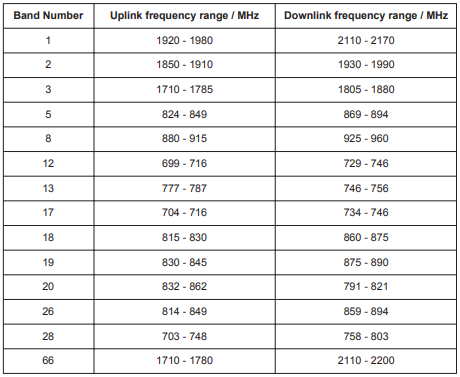
\includegraphics[width=\textwidth]{pict/R13_freq4LTE.png}
    \caption{LTE frequency bands in Release 13 \cite{NB_IoT-rohde}}
    \label{fig:R13-freq4lte}
\end{figure}

\subsection*{Deployment options}
NB-IoT supports three deployment modes \cite{NB_IoT-rohde, Masek2021, ericsson-tech-review}:
\begin{itemize}
    \item Standalone mode: This mode utilizes a standalone 200 kHz carrier in the GSM frequencies.
    \item Guard-band mode: This mode utilizes unused resource blocks within an LTE carrier's guard-band 
    \item In-band mode: This mode utilizes a resource block within an LTE carrier.
\end{itemize}

Fig.\ref{fig:nb-iot-modes} depicts the three deployment modes.
\begin{figure}[h!]
    \centering
    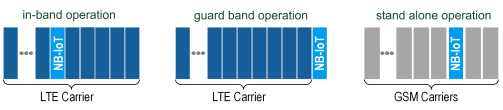
\includegraphics[width=\textwidth]{pict/nb-iot-modes.png}
    \caption{LTE frequency bands in Release 13 \cite{NB_IoT-rohde}}
    \label{fig:nb-iot-modes}
\end{figure}

\section{The NB-IoT network protocol}

